% !TeX program = xelatex
\documentclass[10pt]{beamer}

\usetheme{metropolis}

\usepackage{pgfplots}
\usepgfplotslibrary{fillbetween}
\usepackage{pgfopts}
\usepackage{amsmath}
\usepackage{structuralanalysis}
\usepackage{tikz}
\usepackage{tikz-3dplot}
\usepackage{chngcntr}
\usepackage{wasysym}
\usepackage{mathtools}
\usepackage{alphalph}
\usepackage{xcolor}
\usepackage[showdow=false, en-US]{datetime2}
\usepackage{hyperref}

\newcommand{\highlight}[1]{%
	\colorbox{red!50}{$\displaystyle#1$}}

\setcounter{lecture}{22}
\counterwithin{equation}{lecture}
\makeatletter
\def\user@resume{resume}
\def\user@intermezzo{intermezzo}
%
\newcounter{previousequation}
\newcounter{lastsubequation}
\newcounter{savedparentequation}
\setcounter{savedparentequation}{1}
% 
\renewenvironment{subequations}[1][]{%
	\def\user@decides{#1}%
	\setcounter{previousequation}{\value{equation}}%
	\ifx\user@decides\user@resume 
	\setcounter{equation}{\value{savedparentequation}}%
	\else  
	\ifx\user@decides\user@intermezzo
	\refstepcounter{equation}%
	\else
	\setcounter{lastsubequation}{0}%
	\refstepcounter{equation}%
	\fi\fi
	\protected@edef\theHparentequation{%
		\@ifundefined {theHequation}\theequation \theHequation}%
	\protected@edef\theparentequation{\theequation}%
	\setcounter{parentequation}{\value{equation}}%
	\ifx\user@decides\user@resume 
	\setcounter{equation}{\value{lastsubequation}}%
	\else
	\setcounter{equation}{0}%
	\fi
	\def\theequation  {\theparentequation  \alph{equation}}%
	\def\theHequation {\theHparentequation \alph{equation}}%
	\ignorespaces
}{%
%  \arabic{equation};\arabic{savedparentequation};\arabic{lastsubequation}
\ifx\user@decides\user@resume
\setcounter{lastsubequation}{\value{equation}}%
\setcounter{equation}{\value{previousequation}}%
\else
\ifx\user@decides\user@intermezzo
\setcounter{equation}{\value{parentequation}}%
\else
\setcounter{lastsubequation}{\value{equation}}%
\setcounter{savedparentequation}{\value{parentequation}}%
\setcounter{equation}{\value{parentequation}}%
\fi\fi
%  \arabic{equation};\arabic{savedparentequation};\arabic{lastsubequation}
\ignorespacesafterend
}
\makeatother
\title{AE 737 - Mechanics of Damage Tolerance}
\subtitle{Lecture \arabic{lecture}}
\date{Last Updated: \today\ at \DTMcurrenttime}
\author{Dr. Nicholas Smith}
\institute{Wichita State University, Department of Aerospace Engineering}
% \titlegraphic{\hfill\includegraphics[height=1.5cm]{logo/logo}}

\begin{document}
	
	\maketitle
	\begin{frame}{schedule}
		\begin{itemize}
			\item 14 Apr - Exam Review
			\item 19 Apr - Damage Tolerance, Homework 8 Due
			\item 21 Apr - Exam 2
			\item 26 Apr - Exam Solutions, Damage Tolerance
			\item 28 Apr - SPTE, AFGROW, Finite Elements
			%		\item 3 May - Finite Elements
			%		\item 5 May - Non-Destructive Testing, Composites, Final Project Due May 10
		\end{itemize}
	\end{frame}
	
	\begin{frame}
		\frametitle{outline}
		\setbeamertemplate{section in toc}[sections numbered]
		\tableofcontents[hideallsubsections]
	\end{frame}

	\section{crack growth retardation}
	
	\begin{frame}{crack growth retardation}
		\begin{itemize}[<+->]
			\item When an overload is applied, the plastic zone is larger
			\item This zone has residual compressive stresses, which slow crack growth until the crack grows beyond this over-sized plastic zone
			\item We will discuss three retardation models, but no model has been shown to be perfect in all cases
			\item The Wheeler method reduces $da/dN$, the Willenborg model reduces $\Delta K$, and the Closure model increases $R$ (increases $\sigma_{min}$)
		\end{itemize}
	\end{frame}
	
	\begin{frame}{wheeler retardation}
		\begin{itemize}[<+->]
			\item As long as crack is within overload plastic zone, we scale $da/dN$ by some $\phi$
			\item[] \begin{equation}
			(a_i + r_{pi}) = (a_{ol} + r_{pol})
			\end{equation}
			\item And $\phi$ is given by
			\begin{equation}
			\phi_i = \left[\frac{r_{pi}}{a_{ol}+r_{pol}-a_i}\right]^m
			\end{equation}
			\item and the constant, $m$ is to be determined experimentally
		\end{itemize}
	\end{frame}
	
	\begin{frame}{wheeler example}
		
	\end{frame}
	
	\begin{frame}{willenborg retardation}
		\begin{itemize}[<+->]
			\item Once again, we consider that retardation occurs when $(a_i + r_{pi}) = (a_{ol} + r_{pol})$
			\item Willenborg assumes that the residual compressive stress in the plastic zone creates an effective, $K_{max,eff}$, where $K_{max,eff} = K_{max} - K_{comp}$
			\item The effective stress intensity factor is given by
			\begin{equation}
			K_{max,eff} = K_{max,i} - \left[K_{max,OL}\sqrt{1-\frac{\Delta a_i}{r_{pol}}} - K_{max,i} \right]
			\end{equation} 
		\end{itemize}
	\end{frame}
	
	\begin{frame}{gallagher and hughes correction}
		\begin{itemize}[<+->]
			\item Galagher and Hughes observed that the Willenborg model stops cracks when they still propagate
			\item They proposed a correction to the model
			\item[] \begin{equation}
			K_{max,eff} = K_{max,i} - \phi_i\left[K_{max,OL}\sqrt{1-\frac{\Delta a_i}{r_{pol}}} - K_{max,i} \right]
			\end{equation} 
			\item And the correction factor, $\phi_i$ is given by
			\begin{equation}
			\phi_i = \frac{1-K_{TH}/K_{max,i}}{s_{ol}-1}
			\end{equation}
		\end{itemize}
	\end{frame}
	
	\begin{frame}{willenborg example}
		
	\end{frame}
	
	\begin{frame}{closure model}
		\begin{itemize}[<+->]
			\item Once again, we consider that retardation occurs when $(a_i + r_{pi}) = (a_{ol} + r_{pol})$
			\item Within the overloaded plastic zone, the opening stress required can be expressed as
			\begin{equation}
			\sigma_{OP} = \sigma_{max} (1-(1-C_{f0})(1+0.6R)(1-R))
			\end{equation}
			\item Commonly this is expressed using the Closure Factor, $C_f$
			\item[] \begin{equation}
			C_f = \frac{\sigma_{OP}}{\sigma_{max}} = (1-(1-C_{f0})(1+0.6R)(1-R))
			\end{equation}
			\item Where $C_{f0}$ is the value of the Closure Factor at $R=0$
		\end{itemize}
	\end{frame}
	
	\begin{frame}{closure model}
		\begin{itemize}[<+->]
			\item When using the closure model, we replace $R$ with $C_f$
			\item If the model we are using is in terms of $\Delta K$ we will also need to use $\Delta K = (1-C_f) K_{max}$
		\end{itemize}
	\end{frame}
	
	\begin{frame}{closure example}
		
	\end{frame}
	
	\begin{frame}{compressive under-loads}
		\begin{itemize}[<+->]
			\item Just as a tensile "overload" retards crack growth, we might expect a compressive "underload" to accelerate crack growth
			\item This effect is not usually modeled for a few reasons
			\begin{enumerate}
				\item Compressive underloads are uncommon in airframes
				\item The acceleration effect is minimal
				\item Analysis is generally adjusted with experimental data, so acceleration can be built in to current model
				\item Structures with large compressive loads are not generally subject to crack propagation problems
			\end{enumerate}
		\end{itemize}
	\end{frame}

\section{exam 2}

\begin{frame}{exam 2}
	\begin{itemize}[<+->]
		\item 5 questions
		\item Bring calculator
		\item Closed note/closed book
		\item Make sure you can integrate the Paris Law equation (see Homework 8 problems 1 and 2)
		\item No table look-ups (stress intensity factors, paris/walker law constants will be given in problem)
	\end{itemize}
\end{frame}

\section{stress based fatigue}

\begin{frame}{stress based fatigue}
	\begin{itemize}[<+->]
		\item Has the simplest analysis of any fatigue analysis
		\item Very good for high cycle fatigue (i.e. low stress fatigue)
		\item High cycle fatigue means there is less plasticity
		\item Typically starts between $10^2 - 10^4$ cycles
		\item This point varies by material, but can be found using strain-based fatigue analysis
	\end{itemize}
\end{frame}

\begin{frame}{constant amplitude stressing}
	\begin{figure}
		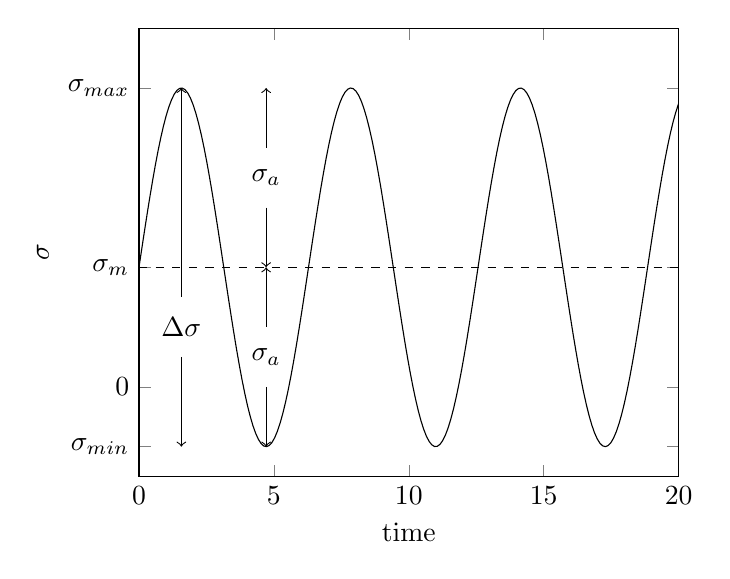
\begin{tikzpicture}
		\begin{axis}[
		domain=0:20,
		samples=200,
		xmin=0,   xmax=20,
		ymin=-3,   ymax=12,
		ylabel=$\sigma$,
		xlabel=time,
		ytick={-2, 0, 4, 10},
		yticklabels={$\sigma_{min}$, 0, $\sigma_m$, $\sigma_{max}$}]
		\addplot [color=black,mark=none] {6*sin(deg(x)) + 4};
		\addplot [color=black,style=dashed,mark=none] coordinates { (0,4) (20,4)};
		\draw[<-] (axis cs: 3.14159/2,10) -- (axis cs: 3.14159/2,3);
		\draw[->] (axis cs: 3.14159/2,1) -- (axis cs: 3.14159/2,-2);
		\draw node at (axis cs: 3.14159/2,2) {$\Delta \sigma$};
		\draw[<-] (axis cs: 3*3.14159/2,4) -- (axis cs: 3*3.14159/2,2);
		\draw[->] (axis cs: 3*3.14159/2,0) -- (axis cs: 3*3.14159/2,-2);
		\draw node at (axis cs: 3*3.14159/2,1) {$\sigma_a$};
		\draw[<-] (axis cs: 3*3.14159/2,10) -- (axis cs: 3*3.14159/2,8);
		\draw[->] (axis cs: 3*3.14159/2,6) -- (axis cs: 3*3.14159/2,4);
		\draw node at (axis cs: 3*3.14159/2,7) {$\sigma_a$};
		\end{axis}
		\end{tikzpicture}
	\end{figure}
\end{frame}

\begin{frame}{constant amplitude stressing}
	\begin{itemize}[<+->]
		\item $\Delta \sigma$ is known as the stress range, and is the difference between max and min stress
		\item $\sigma_m$ is the mean stress, and can sometimes be zero, but this is not always the case
		\item $\sigma_a$ is the stress amplitude, and is the variation about the mean
		\item We can express all of these in terms of the maximum and minimum stress
		\begin{align}
		\Delta \sigma &= \sigma_{max} - \sigma_{min}\\
		\sigma_m &= \frac{\sigma_{max} + \sigma_{min}}{2}\\
		\sigma_a &= \frac{\sigma_{max}- \sigma_{min}}{2}
		\end{align}
	\end{itemize}
\end{frame}

\begin{frame}{constant amplitude stressing}
	\begin{itemize}[<+->]
		\item It is also common to describe some ratios
		\item The stress ratio, $R$ is defined as
		\begin{equation}
		R = \frac{\sigma_{min}}{\sigma_{max}}
		\end{equation}
		\item And the amplitude ratio, $A$ is defined as
		\begin{equation}
		A = \frac{\sigma_a}{\sigma_m}
		\end{equation}
	\end{itemize}
\end{frame}

\begin{frame}{useful relations}
	\begin{itemize}
		\item There are some useful relationships between the above equations
		\begin{subequations}
			\begin{align}
			\Delta \sigma &= 2 \sigma_a = \sigma_{max}(1-R)\\
			\sigma_m &= \frac{\sigma_{max}}{2}(1+R)\\
			R &= \frac{1-A}{1+A}\\
			A &= \frac{1-R}{1+R}
			\end{align}
		\end{subequations}
	\end{itemize}
\end{frame}

\begin{frame}{practical considerations}
	\begin{itemize}[<+->]
		\item High cycle fatigue requires a lot of testing
		\item Usually for very high cycle fatigue some form of rotating beam test machine is used
		\item Rotating 4-point bend is one of the most common modern methods
		\item Tensile test machines can be used, but require much more time
	\end{itemize}
\end{frame}

\begin{frame}{rotating four-point bend}
	\begin{figure}
		\centering
		\includegraphics[width=0.7\linewidth]{../Figures/Rotating_Bending_Machine}
		\caption{Four-point bend gives uniform stress (along top and bottom surfaces)}
		\label{fig:Rotating_Bending_Machine}
	\end{figure}
\end{frame}

\begin{frame}{stress life curves}
	\begin{itemize}[<+->]
		\item Stress-life curves, or S-N curves, are generated from test data to predict the number of cycles to failure
		\item In general, one set (or family) of S-N curves is generated using the same $\sigma_m$
		\item Usually $S_a$ (the nominal stress equivalent of $\sigma_a$) is plotted versus $N$ (the number of cycles)
	\end{itemize}
\end{frame}

\begin{frame}{stress life curves}
	\begin{itemize}[<+->]
		\item Each individual point on an S-N curve represents one fatigue experiment
		\item To find enough data to form statistical significance, as well as to fit a curve across all levels of fatigue is very time-consuming
		\item In the following plot, if only one test was performed for each point, the total number of cycles tested would be about $7.3x10^7$
		\item For a 100 Hz machine, this represents over 200 hours of consecutive testing
		\item Each repetition would further increase the test time required
	\end{itemize}
\end{frame}

\begin{frame}{stress life curves}
	\begin{tikzpicture}
	\begin{axis}[%
	xlabel={$N_f$ (cycles to failure)},%
	ylabel={$S_a$ (MPa)}]
	\addplot[only marks] coordinates {
		(50043.42952596336,304.3384885916487)
		(61810.2778157969,275.4565502529583)
		(64649.06882505588,262.997448795745)
		(169586.85224960672,247.7449948831778)
		(565161.8625105635,233.04313985499925)
		(761338.8628672551,220.14010003026843)
		(1579862.092639026,191.8692976260827)
		(3173264.1073141545,178.55402931722847)
		(3682937.77739026,205.51896106891124)
		(9552328.626265539,185.27652459677992)
		(18242638.367873847,164.96778564118816)
		(35011737.76351732,165.60774874241474)
	};
	\end{axis}
	\end{tikzpicture}
\end{frame}

\begin{frame}{stress life curves}
	\begin{itemize}[<+->]
		\item On a linear scale, the data appear not to agree well with any standard fit
		\item It is also very difficult to differentiate between low-cycle fatigue failure stresses
		\item Instead S-N curves are often plotted on a semi-log or log-log scale, so pay attention to the axes
	\end{itemize}
\end{frame}

\begin{frame}{stress life curves}
	\begin{tikzpicture}
	\begin{axis}[%
	xmode=log,%
	xlabel={$N_f$ (cycles to failure)},%
	ylabel={$S_a$ (MPa)}]
	\addplot[only marks] coordinates {
		(50043.42952596336,304.3384885916487)
		(61810.2778157969,275.4565502529583)
		(64649.06882505588,262.997448795745)
		(169586.85224960672,247.7449948831778)
		(565161.8625105635,233.04313985499925)
		(761338.8628672551,220.14010003026843)
		(1579862.092639026,191.8692976260827)
		(3173264.1073141545,178.55402931722847)
		(3682937.77739026,205.51896106891124)
		(9552328.626265539,185.27652459677992)
		(18242638.367873847,164.96778564118816)
		(35011737.76351732,165.60774874241474)
	};
	\end{axis}
	\end{tikzpicture}
\end{frame}

\begin{frame}{curve fits}
	\begin{itemize}[<+->]
		\item If the curve is nearly linear on a log-linear plot, we use the following form to fit the data
		\item \begin{equation}
		\sigma_a = C + D \log N_f
		\end{equation}
		\item When the data are instead linear on a log-log scale, the following form is generally used
		\item \begin{equation}
		\sigma_a = \sigma_f^\prime \left(2N_f\right)^b
		\end{equation}
		\item $\sigma_f^\prime$ and $b$ are often considered material properties and can often be looked up on a table (p. 235)
	\end{itemize}
\end{frame}

\begin{frame}{stress life curves}
	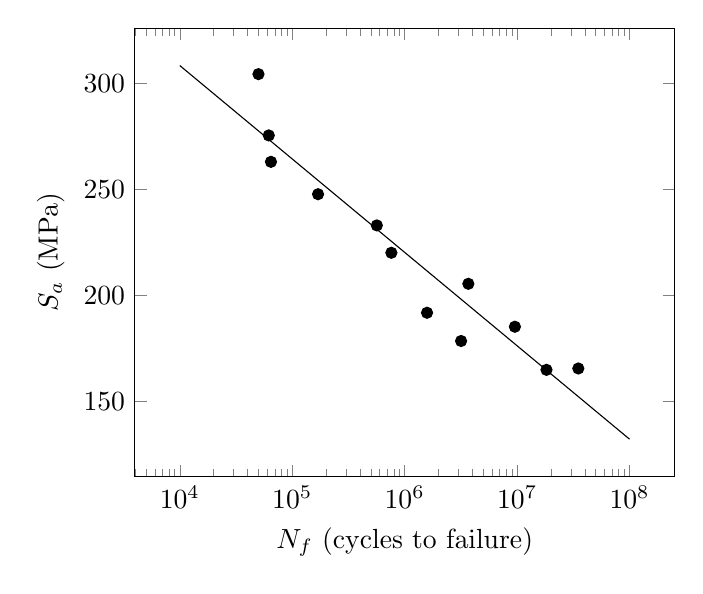
\begin{tikzpicture}
	\begin{axis}[%
	xmode=log,%
	domain=1e4:1e8,%
	samples=200,%
	xlabel={$N_f$ (cycles to failure)},%
	ylabel={$S_a$ (MPa)}]
	\addplot[only marks] coordinates {
		(50043.42952596336,304.3384885916487)
		(61810.2778157969,275.4565502529583)
		(64649.06882505588,262.997448795745)
		(169586.85224960672,247.7449948831778)
		(565161.8625105635,233.04313985499925)
		(761338.8628672551,220.14010003026843)
		(1579862.092639026,191.8692976260827)
		(3173264.1073141545,178.55402931722847)
		(3682937.77739026,205.51896106891124)
		(9552328.626265539,185.27652459677992)
		(18242638.367873847,164.96778564118816)
		(35011737.76351732,165.60774874241474)
	};
	\addplot[no markers] {484.47 - 19.12*ln(x)};
	\end{axis}
	\end{tikzpicture}
\end{frame}

\begin{frame}{fatigue limit}
	\begin{itemize}[<+->]
		\item The fatigue limit, or endurance limit, is a feature of some materials where below a certain stress, no fatigue failure is observed
		\item Below the fatigue limit, this material is considered to have infinite life
		\item This most notably occurs in plain-carbon and low-alloy steels
		\item In these materials, $\sigma_e$ is considered to be a material property
		\item This phenomenon is not typical of aluminum or copper alloys, but is sometimes arbitrarily assigned using whatever the failure stress is at some large number of cycles ($10^7$ or $10^8$)
	\end{itemize}
\end{frame}

\begin{frame}{fatigue limit}
	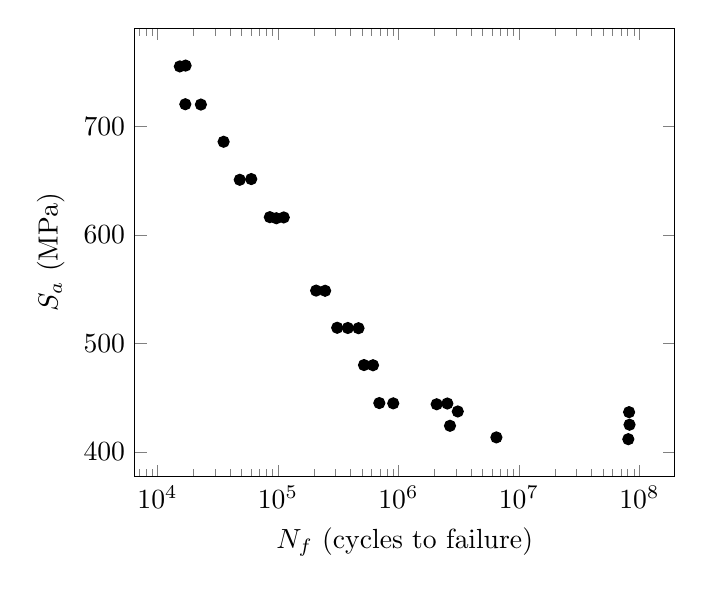
\begin{tikzpicture}
	\begin{axis}[%
	xmode=log,%
	domain=1e3:1e8,%
	samples=200,%
	xlabel={$N_f$ (cycles to failure)},%
	ylabel={$S_a$ (MPa)}]
	\addplot[only marks] coordinates {
		(15335.57305076729,755.3980800096908)
		(17120.563873524803,756.1781896368977)
		(17030.666340686137,720.548741709821)
		(22930.156230029723,720.2495381726781)
		(35394.72596452449,685.9598437358045)
		(48178.50680065504,650.9057872263105)
		(60015.34650935311,651.5756639714122)
		(85619.60323966984,616.4743647981587)
		(96991.95509887673,615.4580418521547)
		(111725.20919888247,616.2066563701887)
		(310167.4766824342,514.5113715514369)
		(380171.36929461616,514.3066533418128)
		(465974.9357903219,514.1019351321886)
		(207329.98874026354,548.7695708791375)
		(246290.6168802425,548.5963477786863)
		(517751.44153305655,480.1429393416311)
		(615045.2363433094,479.96971624117987)
		(693804.9505813519,445.1046303867236)
		(905347.6109897072,444.8369219587535)
		(2075614.3484015197,444.00230156567034)
		(2545405.291185992,444.68792586535835)
		(3106869.8968525752,437.3604675812362)
		(2677489.704626086,424.14705793283065)
		(6497638.107517564,413.4556797189666)
		(82022604.86227266,436.74025620059956)
		(82752208.82434484,425.1500560249538)
		(80830258.5708036,411.81066593985645)
	};
	\end{axis}
	\end{tikzpicture}
\end{frame}

\begin{frame}{effect of variable amplitude}
	\begin{itemize}[<+->]
		\item We know that variable loads can often occur in real scenarios, but how can we model the effect?
		\item Miner's Rule is often used to approximate the effect of variable amplitude load
		\item We consider each load amplitude (and the number of cycles at that amplitude) as having used up a percentage of a part's life
		\item[] \begin{equation}
		\frac{N_1}{N_{f1}} + \frac{N_2}{N_{f2}} + \frac{N_3}{N_{f3}} + ... = \sum \frac{N_i}{N_{fi}} = 1
		\end{equation}
	\end{itemize}
\end{frame}

\begin{frame}{effect of variable amplitude}
	\begin{itemize}[<+->]
		\item Often there are "blocks" of variable amplitude loads which repeat
		\item A typical flight cycle is a good example of this
		\item A flight will have working loads, vibrations, as well as storms/turbulence, but each flight should have similar loading
		\item If we call the number of "block" $B$ then we have
		\item[] \begin{equation}
		B \left[\sum \frac{N_i}{N_{if}}\right]_{rep} = 1
		\end{equation}
	\end{itemize}
\end{frame}

\begin{frame}{mean stress}
	\begin{itemize}[<+->]
		\item Since mean stress has an effect on fatigue life, sometimes a family of S-N curves at varying mean stress values is created
		\item S-N curves for these are reported in different ways, but commonly $\sigma_{max}$ replaces $\sigma_a$ on the y-axis
		\item One useful way of representing these data, instead of many S-N curves, is a constant-life diagram
		\item It is created by taking points from the S-N curves and plotting a line through constant $N_f$ values
	\end{itemize}
\end{frame}

\begin{frame}{Goodman line}
	\begin{itemize}[<+->]
		\item The first work on this problem was done by Goodman, who proposed the line
		\item[] \begin{equation}
		\frac{\sigma_a}{\sigma_{ar}} + \frac{\sigma_m}{\sigma_u} = 1
		\end{equation}
		\item This equation can also be used for fatigue limits, since they are just a point on the S-N curves
		\item[] \begin{equation}
		\frac{\sigma_e}{\sigma_{er}} + \frac{\sigma_m}{\sigma_u} = 1
		\end{equation}
	\end{itemize}
\end{frame}

\begin{frame}{modifications}
	\begin{itemize}[<+->]
		\item While the Goodman line gives a good approximation to convert non-zero mean stress S-N curves, it is somewhat overly conservative at high mean stresses
		\item It is also non-conservative for negative mean stresses
		\item An alternative fit is known as the Gerber Parabola
		\item[]\begin{equation}
		\frac{\sigma_a}{\sigma_{ar}} + \left(\frac{\sigma_m}{\sigma_u}\right)^2 = 1
		\end{equation}
		\item In general, the Goodman line is a good fit for brittle materials (steels) while the Gerber parabola is a better fit for more ductile materials
	\end{itemize}
\end{frame}

\begin{frame}{modifications}
	\begin{itemize}[<+->]
		\item The Goodman line can also be improved by replacing $\sigma_u$ with the corrected true fracture strength $\tilde{\sigma}_{fB}$ or the constant $\sigma_f^\prime$ from the S-N curve fit
		\item[] \begin{equation}
		\label{eq:morrow}
		\frac{\sigma_a}{\sigma_{ar}} + \frac{\sigma_m}{\sigma_f^\prime} = 1
		\end{equation}
		\item This is known as the Morrow Equation
		\item For steels, $\sigma_f^\prime \approx \tilde{\sigma}_{fB}$, but for aluminums these values can be significantly different, and better agreement is found using $\tilde{\sigma}_{fB}$.
	\end{itemize}
\end{frame}

\begin{frame}{modifications}
	\begin{itemize}[<+->]
		\item One more relationship that has shown particularly good results with aluminum alloys is the Smith, Watson, and Topper equations (SWT)
		\item[] \begin{equation}
		\label{eq:swt}
		\sigma_{ar} = \sqrt{\sigma_{max}\sigma_a}
		\end{equation}
		\item In general, it is best to use a form that matches your data
		\item If data is lacking, the SWT (\ref{eq:swt}) and Morrow (\ref{eq:morrow}) equations generally provide the best fit
	\end{itemize}
\end{frame}

\begin{frame}{general stress}
	\begin{itemize}[<+->]
		\item Often combined loads from different sources introduce stresses which are not uni-axial
		\item For ductile materials, good agreement has been found using an effective stress amplitude, similar to the octahedral shear yield criterion
		\item[] \begin{equation}
		\bar{\sigma}_a = \frac{1}{\sqrt{2}}\sqrt{(\sigma_{xa}-\sigma_{ya})^2 + (\sigma_{ya}-\sigma_{za})^2 + (\sigma_{za}-\sigma_{xa})^2 + 6(\tau_{xy}^2 + \tau_{yz}^2 + \tau_{zx}^2)}
		\end{equation}
		\item The effective mean stress is given by
		\item[] \begin{equation}
		\bar{\sigma}_m = \bar{\sigma}_{xm} + \bar{\sigma}_{ym} + \bar{\sigma}_{zm}
		\end{equation}
	\end{itemize}
\end{frame}

\begin{frame}{notch effects}
	\begin{itemize}[<+->]
		\item In this discussion, we use "notch" to refer to any geometric feature that increases the local stress (such as holes, fillets, grooves, etc.)
		\item We discussed notches and stress concentration factors in terms of stress concentration factors
		\item In our fatigue notation, $\sigma_{max} = K_t S$
		\item This relates local stress to the average, nominal stress
		\item The stress intensity factor can be used to characterize the "strength" of a notch
	\end{itemize}
\end{frame}

\begin{frame}{notch effects}
	\begin{itemize}[<+->]
		\item We might expect the fatigue life of a notched specimen to be similar to a pristine specimen with $S_{a,pristine} = \sigma_{max,notched}$
		\item If we look at actual test data, however, this estimate would be overly conservative
		\item Even when the stress is adjusted for some fatigue notch factor, $k_f$, it is only valid at longer cycles ($N_f > 10^6$)
		\item[] \begin{equation}
		k_f = \frac{\sigma_{ar}}{S_{ar}}
		\end{equation}
		\item Notches will have different effects, largely depending on their radius.
		\item The maximum possible fatigue notch factor is $k_f = k_t$
	\end{itemize}
\end{frame}

\begin{frame}{notch sensitivity factor}
	\begin{itemize}[<+->]
		\item To avoid generating fatigue data for every possible notch configuration, some empirical relationships have been developed
		\item A useful concept in these methods is the notch sensitivity factor
		\item[] \begin{equation}
		q = \frac{k_f - 1}{k_t -1}
		\end{equation}
		\item When $k_f = 1$, $q=0$, in which case the notch has no effect
		\item When $k_f = k_t$, $q=1$, in which case the notch has its maximum effect
	\end{itemize}
\end{frame}

\begin{frame}{peterson notch sensitivity}
	\begin{itemize}[<+->]
		\item Peterson developed the following relationship
		\item[] \begin{equation}
		q = \frac{1}{1+\frac{\alpha}{\rho}}
		\end{equation}
		\item Where $\rho$ is the radius of the notch
		\item $\alpha$ is a material property
		\item[]
		\begin{table}
			\caption{Table of $\alpha$ values for Peterson notch sensitivity equation}
			\begin{tabular}{ccc}
				Material & $\alpha$ (mm) & $\alpha$ (in) \\ 
				\hline Aluminum alloys & 0.51 & 0.02 \\ 
				Annealed or low-carbon steels & 0.25 & 0.01 \\ 
				Quenched and tempered steels & 0.064 & 0.0025 
			\end{tabular} 
		\end{table}
	\end{itemize}
\end{frame}

\begin{frame}{peterson notch sensitivy}
	\begin{itemize}[<+->]
		\item For high-strength steels, a more specific $\alpha$ estimate can be found
		\begin{align}
		\alpha &= 0.025 \left(\frac{2070 }{\sigma_u}\right)^{1.8} & \text{mm} & \qquad \sigma_u \ge 550 \text{ MPa}\\
		\alpha &= 0.001 \left(\frac{300 }{\sigma_u}\right)^{1.8} & \text{in} & \qquad \sigma_u \ge 80 \text{ ksi}
		\end{align}
		\item $\alpha$ predictions are valid for bending and axial fatigue
		\item For torsion fatigue, a good estimate can be found
		\item[] \begin{equation}
		\alpha_{torsion} = 0.6 \alpha
		\end{equation}
	\end{itemize}
\end{frame}

\section{strain based fatigue}

\begin{frame}{strain based fatigue}
	\begin{itemize}[<+->]
		\item The strain based fatigue method uses local stresses and strains (instead of global, nominal values)
		\item The strain-based method gives greater detail, and validity at lower cycles
		\item It is still valid for high cycle fatigue
		\item Does not include crack growth analysis or fracture mechanics
	\end{itemize}
\end{frame}

\begin{frame}{lines}
	\begin{itemize}[<+->]
		\item If we separate elastic and plastic strains, we notice that the data for elastic and plastic strains are represented by straight lines, in the log-log scale
		\item If we recall the form used for a straight line in log-log plots for S-N curves:
		\item[] \begin{equation}
		\sigma_a = \sigma_f^\prime (2N_f)^b
		\end{equation}
		\item We can convert this to find the elastic component of strain
		\item[] \begin{equation}
		\label{eq:elastic}
		\epsilon_{ea} = \frac{\sigma_f^\prime}{E} (2N_f)^b
		\end{equation}
	\end{itemize}
\end{frame}

\begin{frame}{lines}
	\begin{itemize}[<+->]
		\item We can use the same form with new constants for the plastic component of strain
		\item[]\begin{equation}
		\label{eq:plastic}
		\epsilon_{pa} = \epsilon_f^\prime (2 N_f)^c
		\end{equation}
		\item We can combine \ref{eq:elastic} with \ref{eq:plastic} to find the total strain-life curve
		\item[] \begin{equation}
		\epsilon_a = \frac{\sigma_f^\prime}{E} (2N_f)^b + \epsilon_f^\prime (2 N_f)^c
		\end{equation}
	\end{itemize}
\end{frame}

\begin{frame}{mean stress in strain-based fatigue}
	\begin{itemize}[<+->]
		\item In regions where plastic strain is significant, some applied mean stress is likely to be relaxed through cyclic plastic strain
		\item When the plastic strain is not significant, mean stress will exist
		\item Mean strain does not generally affect fatigue life
	\end{itemize}
\end{frame}

\begin{frame}{morrow approach}
	\begin{itemize}[<+->]
		\item Recall the Morrow approach for mean stress effects from the stress-based method
		\item[]\begin{equation}
		\frac{\sigma_a}{\sigma_{ar}} + \frac{\sigma_m}{\sigma_f^\prime} = 1
		\end{equation}
		\item We can rearrange the equation such that
		\item[]\begin{equation}
		\sigma_a = \sigma_f^\prime\left[\left(1-\frac{\sigma_m}{\sigma_f^\prime}\right)^\frac{1}{b}(2N_f)\right]^b
		\end{equation}
	\end{itemize}
\end{frame}

\begin{frame}{morrow approach}
	\begin{itemize}[<+->]
		\item If we compare to the stress-life equation ($\sigma_a = \sigma_f^\prime(2N_f)^b$), we see that we can replace $N_f$ with
		\item[] \begin{equation}
		\label{eq:nstar}
		N^* = N_f \left(1-\frac{\sigma_m}{\sigma_f^\prime}\right)^\frac{1}{b}
		\end{equation}
		\item We can now substitute $N^*$ for $N_f$ in the strain-life equation to find
		\item[] \begin{equation}
		\epsilon_a = \frac{\sigma_f^\prime}{E} \left(1-\frac{\sigma_m}{\sigma_f^\prime}\right)(2N_f)^b + \epsilon_f^\prime\left(1-\frac{\sigma_m}{\sigma_f^\prime}\right)^\frac{c}{b} (2 N_f)^c
		\end{equation}
	\end{itemize}
\end{frame}

\begin{frame}{morrow approach}
	\begin{itemize}[<+->]
		\item Graphically, we can use the Morrow approach very easily using only the zero-mean stress graph
		\item From the zero-mean stress graph, find the point corresponding to your applied strain
		\item For a non zero mean stress, this point represents $(\epsilon_a, N^*)$, we can now solve for $N_f$ using \ref{eq:nstar}
	\end{itemize}
\end{frame}

\begin{frame}{modified morrow}
	\begin{itemize}[<+->]
		\item While the Morrow equation agrees very well with many data, some are better fit with a modification
		\item In the modified version, it is assumed that the mean stress has no effect on the plastic term
		\item[] \begin{equation}
		\epsilon_a = \frac{\sigma_f^\prime}{E}\left(1-\frac{\sigma_m}{\sigma_f^\prime}\right)(2N_f)^b + \epsilon_f^\prime (2N_f)^c
		\end{equation}
		\item There is no convenient solution method for this form, and it generally must be solved numerically, or plotted with many families of $\sigma_m$
	\end{itemize}
\end{frame}

\begin{frame}{smith watson topper}
	\begin{itemize}[<+->]
		\item The Smith, Watson, and Topper approach assumes that the life for any given state is dependent on the product $\sigma_max \epsilon_a$
		\item After some manipulation, this gives
		\item[] \begin{equation}
		\sigma_{max} \epsilon_a = \frac{\left(\sigma_f^\prime\right)^2}{E}(2N_f)^{2b} + \sigma_f^\prime \epsilon_f^\prime (2N_f)^{b+c}
		\end{equation}
		\item This method can also be solved graphically if a plot of $\sigma_{max} \epsilon_a$ is made using zero-mean data. All we need to do is find the new $\sigma_{max} \epsilon_a$ point to find a new $N_f$
	\end{itemize}
\end{frame}

\begin{frame}{comparison}
	\begin{itemize}[<+->]
		\item All three methods discussed are in general use
		\item The Morrow method is very good for steel
		\item The modified Morrow method gives improved results in many materials
		\item The SWT approach is very good for general use, but is non-conservative with a compressive mean stress
	\end{itemize}
\end{frame}

\section{fracture based fatigue}

\begin{frame}{fracture surface}
	\begin{figure}
		\centering
		\includegraphics[width=0.7\linewidth]{../Figures/fracture_surface}
		\label{fig:fracture_surface}
	\end{figure}
\end{frame}

\begin{frame}{fracture surface}	
	\begin{figure}
		\centering
		\includegraphics[width=0.7\linewidth]{../Figures/Fatigue-Fracture-with-Beachmarks}
		\label{fig:Fatigue-Fracture-with-Beachmarks}
	\end{figure}
\end{frame}

\begin{frame}{crack growth rate}
	\begin{itemize}[<+->]
		\item We can observe that fatigue damage occurs through crack propagation
		\item "cracks" and fracture mechanics have been omitted from all our fatigue discussion thus far
		\item It would be beneficial to predict at what rate a crack will extend
	\end{itemize}
\end{frame}

\begin{frame}{crack growth rate}
	\begin{itemize}[<+->]
		\item Crack growth rate can be measured experimentally 
		\item Using a center-crack specimen, a fatigue load is applied
		\item The crack length is measured and plotted vs. the number of cycles
		\item The slope of this curve ($\frac{da}{dN}$) is then plotted vs. either $K_{I,max}$ or $\Delta K_I$ on a log-log scale
		\item This chart is then commonly divided into three regions
	\end{itemize}
\end{frame}

\begin{frame}{da-dN vs K}	
	\begin{figure}
		\centering
		\includegraphics[width=0.7\linewidth]{../Figures/da-dn}
		\label{fig:da-dn}
	\end{figure}
\end{frame}

\begin{frame}{region I}
	\begin{itemize}[<+->]
		\item In Region I crack growth is very slow and/or difficult to measure
		\item In many cases, da/dN corresponds to the spacing between atoms!
		\item The point at which the da/dN curve intersects the boundary between Region I and Region II is often called the fatigue threshold
		\item Typically 3-15 $\text{ ksi} \sqrt{\text{in}}$ for steel
		\item 3-6 $\text{ ksi} \sqrt{\text{in}}$ for aluminum
	\end{itemize}
\end{frame}

\begin{frame}{region II}
	\begin{itemize}[<+->]
		\item Most important region for general engineering analysis
		\item Once a crack is present, most of the growth and life occurs in Region II
		\item Generally linear in the log-log scale
	\end{itemize}
\end{frame}

\begin{frame}{region III}
	\begin{itemize}[<+->]
		\item Unstable crack growth
		\item Usually neglected (we expect failure before Region III fully develops in actual parts)
		\item Can be significant for parts where we expect high stress and relatively short life
	\end{itemize}
\end{frame}

\begin{frame}{crack growth rate curve}
	\begin{itemize}[<+->]
		\item The crack growth rate curve is considered a material property
		\item The same considerations for thickness apply as with fracture toughness ($K_c$ vs. $K_{Ic}$) 
		\item Is also a function of the load ratio, $R = \sigma_{min}/\sigma_{max}$
	\end{itemize}
\end{frame}

\begin{frame}{R effects}
	\begin{itemize}[<+->]
		\item While the x-axis can be either $\Delta K$ or $K_{max}$, the shape of the data is the same
		\item When we look at the effects of load ratio, $R$, the axis causes some differences on the plot
		\item With $\Delta K$ on the x-axis, increasing $R$ will shift the curve up and to the left, shifting the fatigue threshold and fracture toughness on the graph as well
		\item With $K_{max}$ on the x-axis, increasing $R$ shifts the curve down and to the right, but fatigue threshold and fracture toughness keep same values
		\item In general, $R$ dependence vanishes for $R> 0.8$ or $R<-0.3$. This effect is known as the band width
	\end{itemize}
\end{frame}

\begin{frame}{boeing method for variable amplitude loads}
	\begin{itemize}[<+->]
		\item Whether integrating numerically or analytically, it is time-consuming to consider multiple repeated loads
		\item It is particularly difficult to consider flight loads, which can vary by "mission"
		\item For example, an aircraft may fly three different routes, in no particular order, but with a known percentage of time spent in each route
		\item Traditional methods would use a random mix of each load spectra
		\item The Boeing Method combines each repeatable load spectrum into one single equivalent cycle
	\end{itemize}
\end{frame}

\begin{frame}{boeing method}
	\begin{itemize}[<+->]
		\item The Boeing method is derived by separating the geometry effects from load and material effects in the Boeing-Walker equation.
		\item[] \begin{equation}
		\frac{da}{dN} = \left[\frac{1}{n}\right]\frac{dL}{dN} = 10^{-4} \left[\frac{k_{max}Z}{m_T}\right]^p
		\end{equation}
		\item[] \begin{equation}
		\frac{dL}{dN} = n 10^{-4} \left[\frac{k_{max}Z}{m_T}\right]^p
		\end{equation}
		\item[] \begin{equation}
		\frac{dN}{dL} = \frac{1}{n} 10^{4} \left[\frac{m_T}{k_{max}Z}\right]^p
		\end{equation}
		\item[] \begin{equation}
		\int_{0}^{N}dN = \frac{10^{4}}{n}  \int_{L_0}^{L_f} \left[\frac{m_T}{k_{max}Z}\right]^p dL
		\end{equation}
		\item[] \begin{equation}
		N = 10^{4} \left(\frac{m_t}{z\sigma_{max}}\right)^p  \int_{L_0}^{L_f} \frac{dL}{\left( n\sqrt{\pi L/n}\beta\right)^p}
		\end{equation}
	\end{itemize}
\end{frame}

\begin{frame}{boeing method}
	\begin{itemize}[<+->]
		\item In this form, the term $10^{4} \left(\frac{m_t}{z\sigma_{max}}\right)^p$ is strictly from the applied load and material, while $\int_{L_0}^{L_f} \frac{dL}{\left( n\sqrt{\pi L/n}\beta\right)^p}$ is from geometry
		\item If we now define $G$ to account for crack geometry
		\item[] \begin{equation}
		G = \left[ \int_{L_0}^{L_f} \frac{dL}{\left( n\sqrt{\pi L/n}\beta\right)^p} \right] ^{-1/p}
		\end{equation}
		\item And define $z \sigma_{max} = S$ as the equivalent load spectrum, then we have
		\item[] \begin{equation}
		\label{eq:boeing}
		N = 10^4 \left(\frac{m_t/G}{S}\right)^p
		\end{equation}
		\item Using this method, $G$ is typically looked up from a chart (such as on p. 369)
	\end{itemize}
\end{frame}

\begin{frame}{boeing method}
	\begin{itemize}[<+->]
		\item To replace a repeated load spectrum with an equivalent load, we need to invert the relationship
		\item Equation~\ref{eq:boeing} gives cycles per crack growth, inverting gives crack growth per cycle
		\item[] \begin{equation}
		\text{crack growth per cycle} = 10^{-4} \left(\frac{m_t/G}{S}\right)^{-p}
		\end{equation}
		\item If we consider a general, repeatable "block", we have
		\item[] \begin{equation}
		10^{-4} \left( m_t/G \right)^{-p} \sum_i \left( \frac{1}{z\sigma_{max}} \right)_i^{-p} N_i = 10^{-4} \left( \frac{m_t/G}{S} \right)^{-p}
		\end{equation}
		\item Which simplifies to
		\begin{equation}
		\sum_i \left( z\sigma_{max} \right)_i^{p}N_i = \left( S \right)^{p}
		\end{equation}		
	\end{itemize}
\end{frame}

\begin{frame}{cycle counting}
	\begin{itemize}[<+->]
		\item As illustrated in our previous example, cycle counting method can make a difference for variable amplitude loads
		\item Two common methods for cycle counting that give similar results are known as the "rainflow" and "range-pair" methods
		\item ASTM E1049-85 "Standard Practices for Cycle Counting in Fatigue Analysis"
	\end{itemize}
\end{frame}

\begin{frame}{rain-flow method}
	\begin{enumerate}[<+->]
		\item Read next peak or valley. $S$ is the starting point, $Y$ is the first range, $X$ is the second range
		\item If $X < Y$ advance points ($S$ remains same, $Y$ and $X$ change)
		\item If $X \ge Y$ and $Y$ contains $S$, count $Y$ as 1/2-cycle, discard $S$ and go to 1
		\item If $X \ge Y$ and $Y$ does not contain $S$, count $Y$ as 1 cycle, discard both points in $Y$ and go to 1 ($S$ remains same)
		\item When end of data is reached, count each range as 1/2-cycle
	\end{enumerate}
\end{frame}

\begin{frame}{range-pair method}
	\begin{enumerate}[<+->]
		\item Read next peak or valley. $Y$ is the first range, $X$ is the second range
		\item If $X < Y$ advance points
		\item If $X \ge Y$, count $Y$ as 1 cycle and discard both points in $Y$, go to 1
		\item Remaining cycles are counted backwards from end of history
	\end{enumerate}
\end{frame}
\end{document}
